\newpage

\begin{appendices}

\section{TCGA subtypes}


    
    \begin{figure}[!htb]    
        \centering
    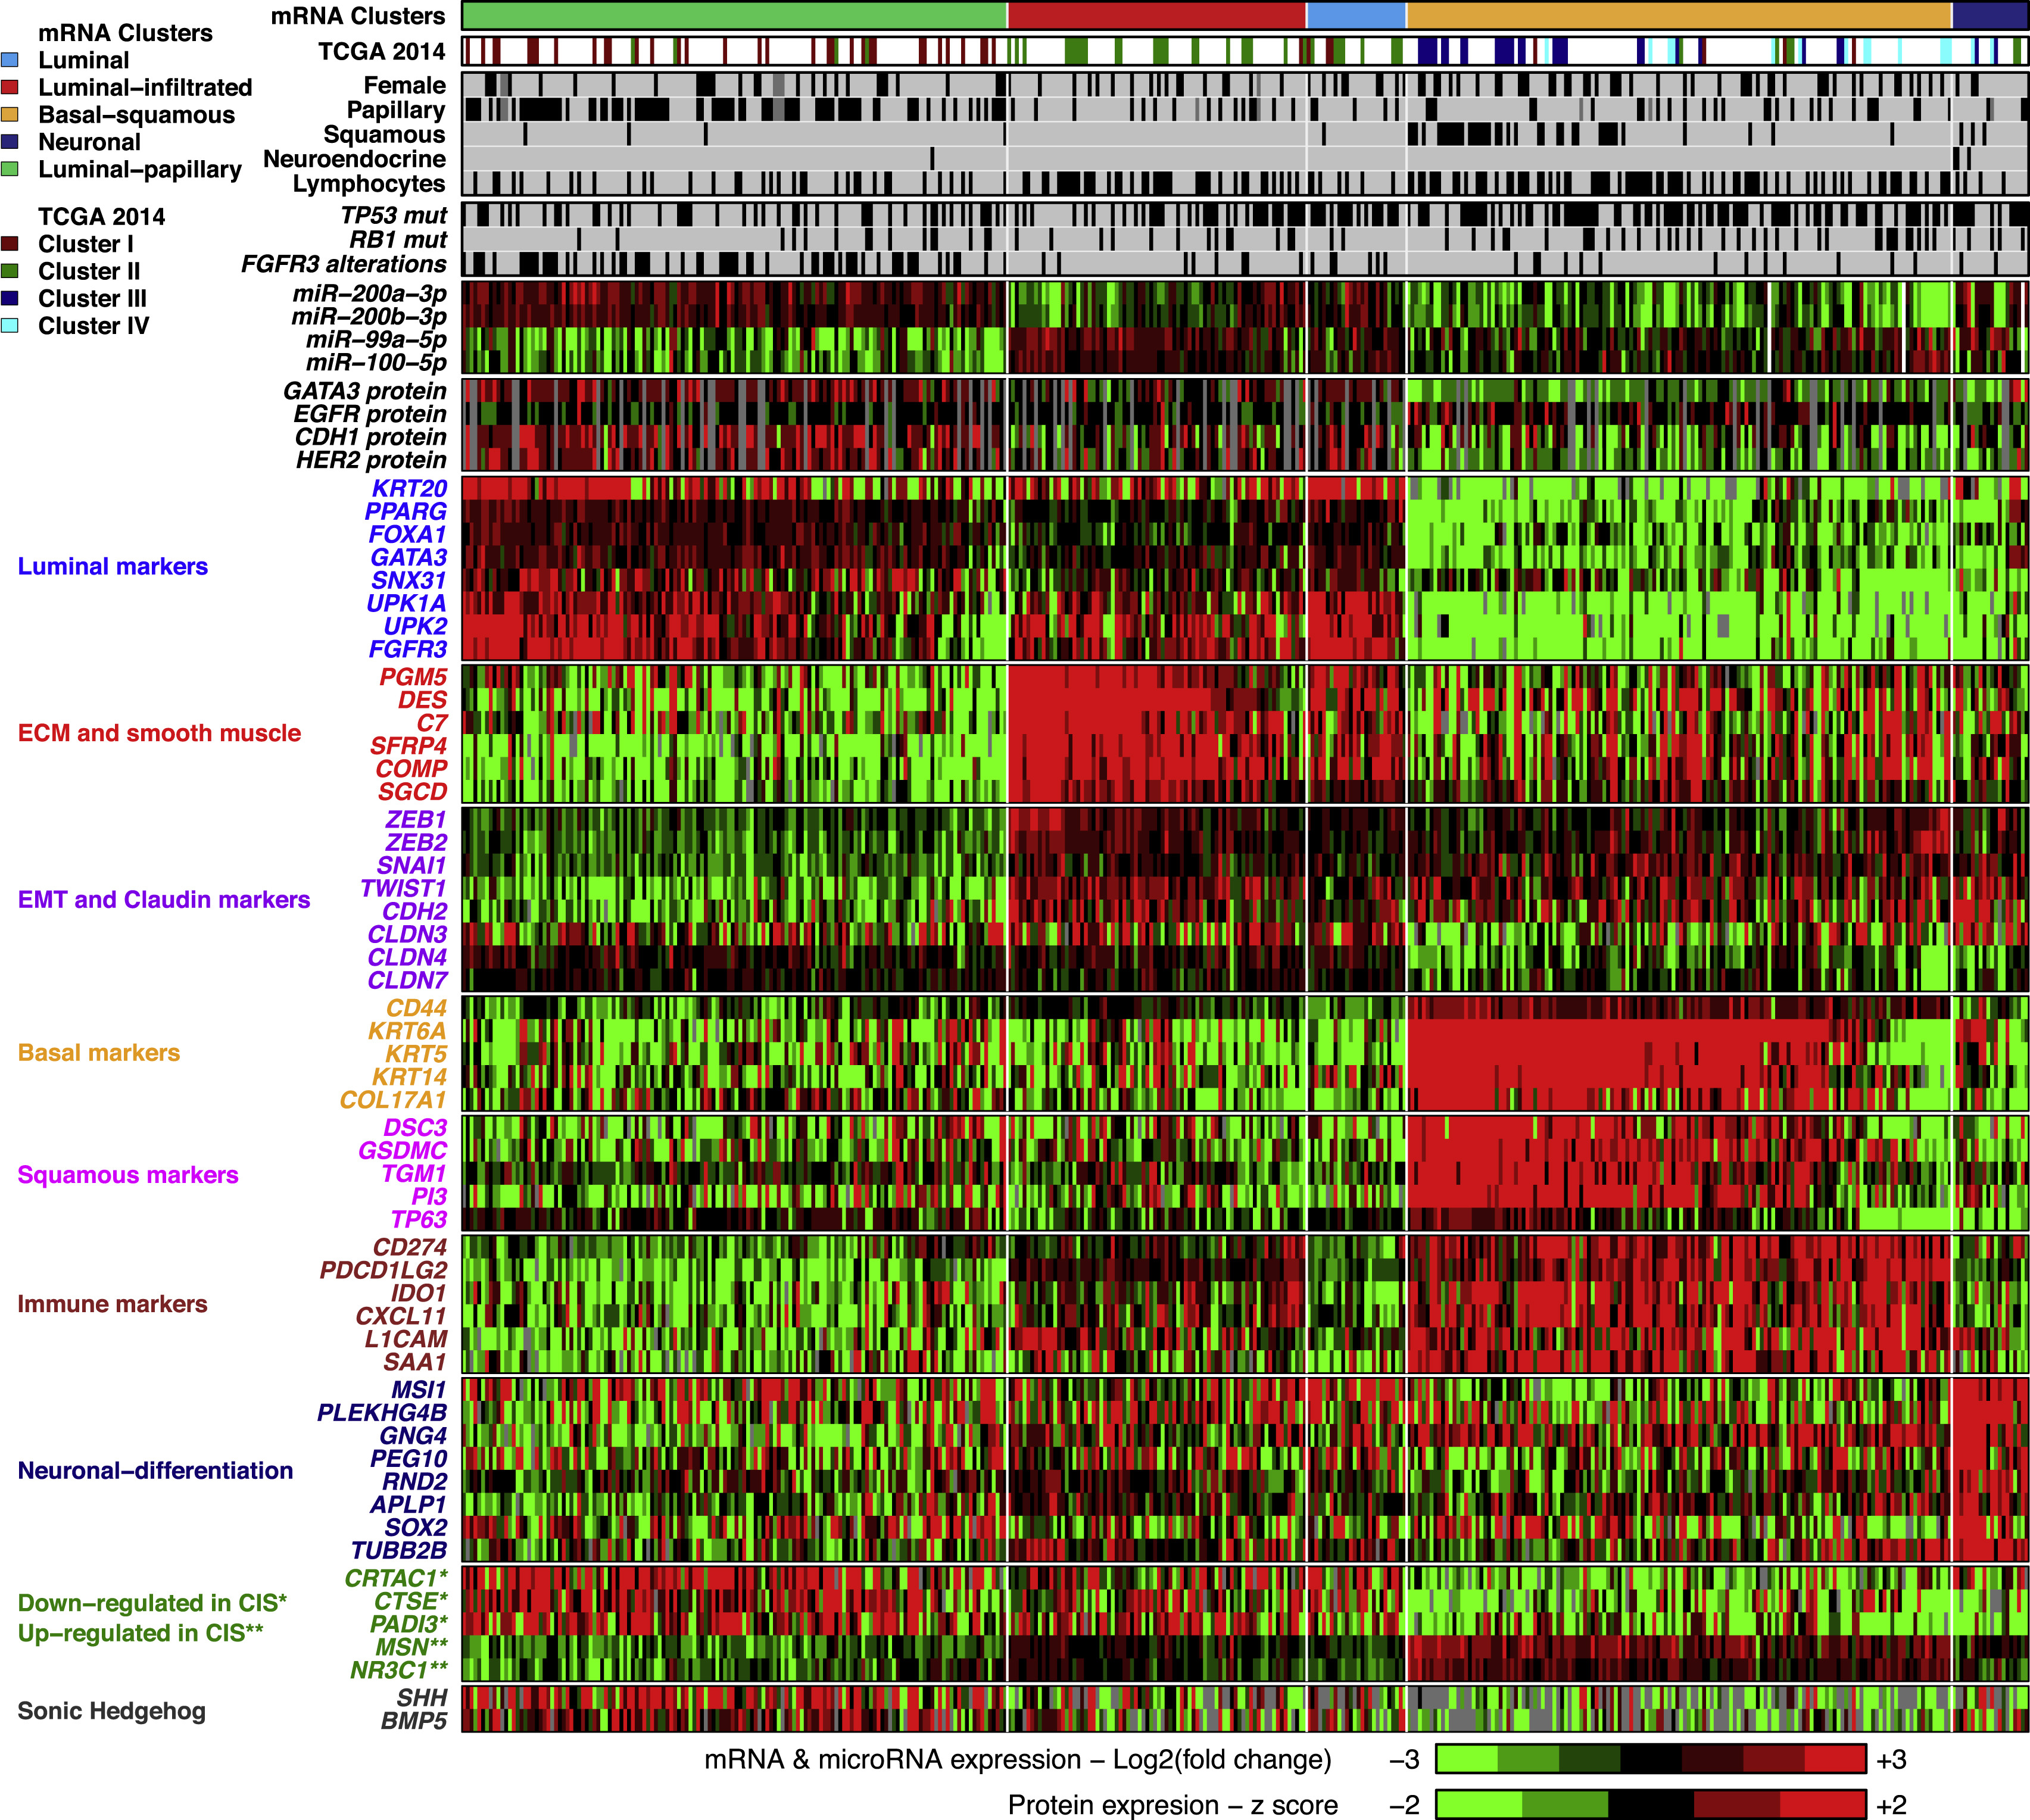
\includegraphics[width=0.9\textwidth,height=0.9\textheight,keepaspectratio]{Sections/Lit_review/Resources/TCGA_2017_subtypes.jpg}
        \caption{Image from \cite{Robertson2017-mg} showing 5 different molecular subtypes found in the MIBC cohort from TCGA. }
        \label{fig:ap:tcga_subtypes}
    \end{figure}


% List of models
\section{List of Models} \label{ap:tables_models}

\begin{small}
    % \KOMAoptions{paper=landscape,pagesize}
    % \begin{table}
      \begin{longtable}[!h]{|p{2.0cm}|c|p{1.5cm}|c|p{2.2cm}|p{6.0cm}|} 
          \hline \multicolumn{1}{|c|}{\textbf{Model}} 
          & \multicolumn{1}{p{1.8cm}|}{\textbf{RNAseq}} 
          & \multicolumn{1}{p{1.5cm}|}{\textbf{Micro-arrays}} 
          & \multicolumn{1}{c|}{\textbf{Mutations}} 
          & \multicolumn{1}{c|}{\textbf{Other}}
          & \multicolumn{1}{c|}{\textbf{Approach}}  \\ \hline  \hline
          \endfirsthead
          
          \endlastfoot    
            \citet{Cava2018-rv} & x &  &  & Pathways & Network/Graph \\ \hline
            GANPA &  & x &  & Protein-protein & Network/Graph \\ \hline
            LEGO & x &  &  &  Pathways  & Network/Graph \\ \hline
            Dendrix &  &  & x &  & Greedy algorithm \& Monte Carlo (MCMC) \\ \hline
            MDPFinder & x &  & x &  &  EA \& optimisation algorithms  \\ \hline
            Neuro-evolution &  & x &  &  & FS-NEAT, feature selection via neuroevolution / supervised \\ \hline
            PICNIC  &  &  & x &  & Pipeline, 4 stages with a range of models \\ \hline
            DriverNet & x &  & x &  & Network/graph \\ \hline
            DawnRank & x &  & x & Gene network &  Network/graph. Built on DriverNet \& using PageRank. \\ \hline
            Memo & x &  & x &  & Network/Graphs, Stats \\ \hline
            iPAC & x &  & x &  &  Stats \& correlations \\ \hline
            Comet  & x &  & x &  & Submatrix, Marko Chain Monte Carlo  \\ \hline
            \citet{Feltes2019-bd} & x & x &  &  & Built on Neuroevolution \\ \hline
            \citet{Palazzo2019-hx} &  &  & x &  & Autoencoders, hierarchical clustering \\ \hline
            \citet{Chaudhary2018-qj} & x &  &  & miRNA, DNA methylation & Autoencoders \\ \hline
            \citet{Ma2019-hk} & x &  &  & miRNA, DNA methylation & Autoencoders \\ \hline
            TCGA clustering & x &  &  &  & Hierarchical clustering \\ \hline
            Consensus clustering & x &  &  &  & Hierarchical clustering \\ \hline
           \citet{Capecci2020-uj} &  & x & x &  & SNN and EA \\ \hline
            MutsigCV &  &  & x &  & Stats \\ \hline
        % \end{tabular}
        \caption{Computational models explored in this literature review with the type of data used and the approaches.}
        \label{tab:data_used}
      \end{longtable}
    \end{small}
    % \KOMAoptions{paper=portrait,pagesize}
    
    \newpage
    \begin{small}
      \begin{longtable}[!h]{|p{2.0cm}|p{2.5cm}|p{3.5cm}|p{3.0cm}|p{5.5cm}|} 
        \hline \multicolumn{1}{|c|}{\textbf{Model}} 
        & \multicolumn{1}{c|}{\textbf{Data used}} 
        & \multicolumn{1}{c|}{\textbf{Datasets}} 
        & \multicolumn{1}{c|}{\textbf{Approach}}
        & \multicolumn{1}{c|}{\textbf{Goal}}  \\ \hline  \hline
        \endfirsthead
        
        \endlastfoot    
          \citet{Cava2018-rv} & Mut & KEGG [5]; TCGA  & Network/ Graph & Establish a connection between GE and functional pathways  \\ \hline
          GANPA & GE  & GSEA; for PPI -HPRD, MINT, DIP, MINT, IntAct & Network/Graph & Breast cancer, asthma, p53 \\ \hline
          LEGO & GE + pathways & KEGG \& others & Network/ Graph & Autism and breast cancer \\ \hline
          Dendrix & GE & TCGA, Thomas et al. & Greedy algorithm, Monte Carlo & Pan-cancer analysis \\ \hline
          MDPFinder & GE + Mut & From Dendrix, TCGA & EA, optimisation aglorithm & Head \& Neck, glioblastoma and ovarian cancer \\ \hline
          Neuro-evolution & GE & Gene Expression Omnibus (GEO) & FS-NEAT, feature selection via neuroevolution / supervised & Leukaemia, breast, and colorectal cancers \\ \hline
          PICNIC  & Mut & TCGA  & Pipeline, 4 stages with a range of models & Multiple cancer types  \\ \hline
          DriverNet & GE + Mut & TCGA, METABRIC, TN and GBM & Network/graph &  Glioblastoma, breast, triple-negative breast, serous ovarian \\ \hline
          DawnRank & GE + Mut & TCGA & Network/graph. Built on DriverNet, using PageRank & Breast, ovarian cancer \\ \hline
          Memo & GE + Mut & TCGA & Network/Graphs, Stats & glioblastoma multiforme (GBM) and ovarian cancer \\ \hline
          iPAC & GE + Mut & Multiple datasets & Stats, correlations & Breast \\ \hline
          Comet  & GE + Mut & TCGA & Submatrix, Marko Chain Monte Carlo & breast \& gastric cancer, glioblastoma, myeloid leukaemia \\ \hline
          \citet{Feltes2019-bd} & GE  & GEO / (Various datasets) & Built on Neuroevolution & Pan-cancer \\ \hline
          \citet{Palazzo2019-hx} & Mut & International Cancer Genome Consortium & Autoencoders, hierarchical clustering & tumor mutation profile analysis \\ \hline
          \citet{Chaudhary2018-qj} & GE + others & TCGA & Autoencoders & Patient survival on liver cancer \\ \hline
          \citet{Ma2019-hk} & GE & TCGA, STRING & Autoencoders &  Bladder and Brain Lower Grade Glioma \\ \hline
          TCGA clustering & GE & TCGA & Hierarchical clustering & Bladder cancer  \\ \hline
          Consensus clustering & GE & TCGA & Hierarchical clustering & Bladder cancer \\ \hline
          \citet{Capecci2020-uj} & GE + Mut & TCGA & SNN and EA & Skin dermatisis  \\ \hline
      \caption{Datasets: Kyoto Encyclopedia of Genes and Genomes (KEGG) \cite{Kanehisa2017-wj}, The Cancer Genome Atlas (TCGA) \cite{Tcga2018-sj}, \citet{Thomas2007-yj} - "High-throughput oncogene mutation profiling in human cancer", The Gene Expression Omnibus (GEO) \cite{ Clough2016-zc, Davis2007-at}, International Cancer Genome Consortium (ICGC) \cite{International_Cancer_Genome_Consortium2010-ca}, Search Tool for Retrieval of Interacting Genes/Proteins(STRING) \cite{Szklarczyk2019-pu}. } 
      \label{tab:approaches}
      \end{longtable}
    \end{small}


% Dendogram example
\section{Dendrogram} \label{ap:dendogram}


\begin{figure}[!htb]                                  
    \centering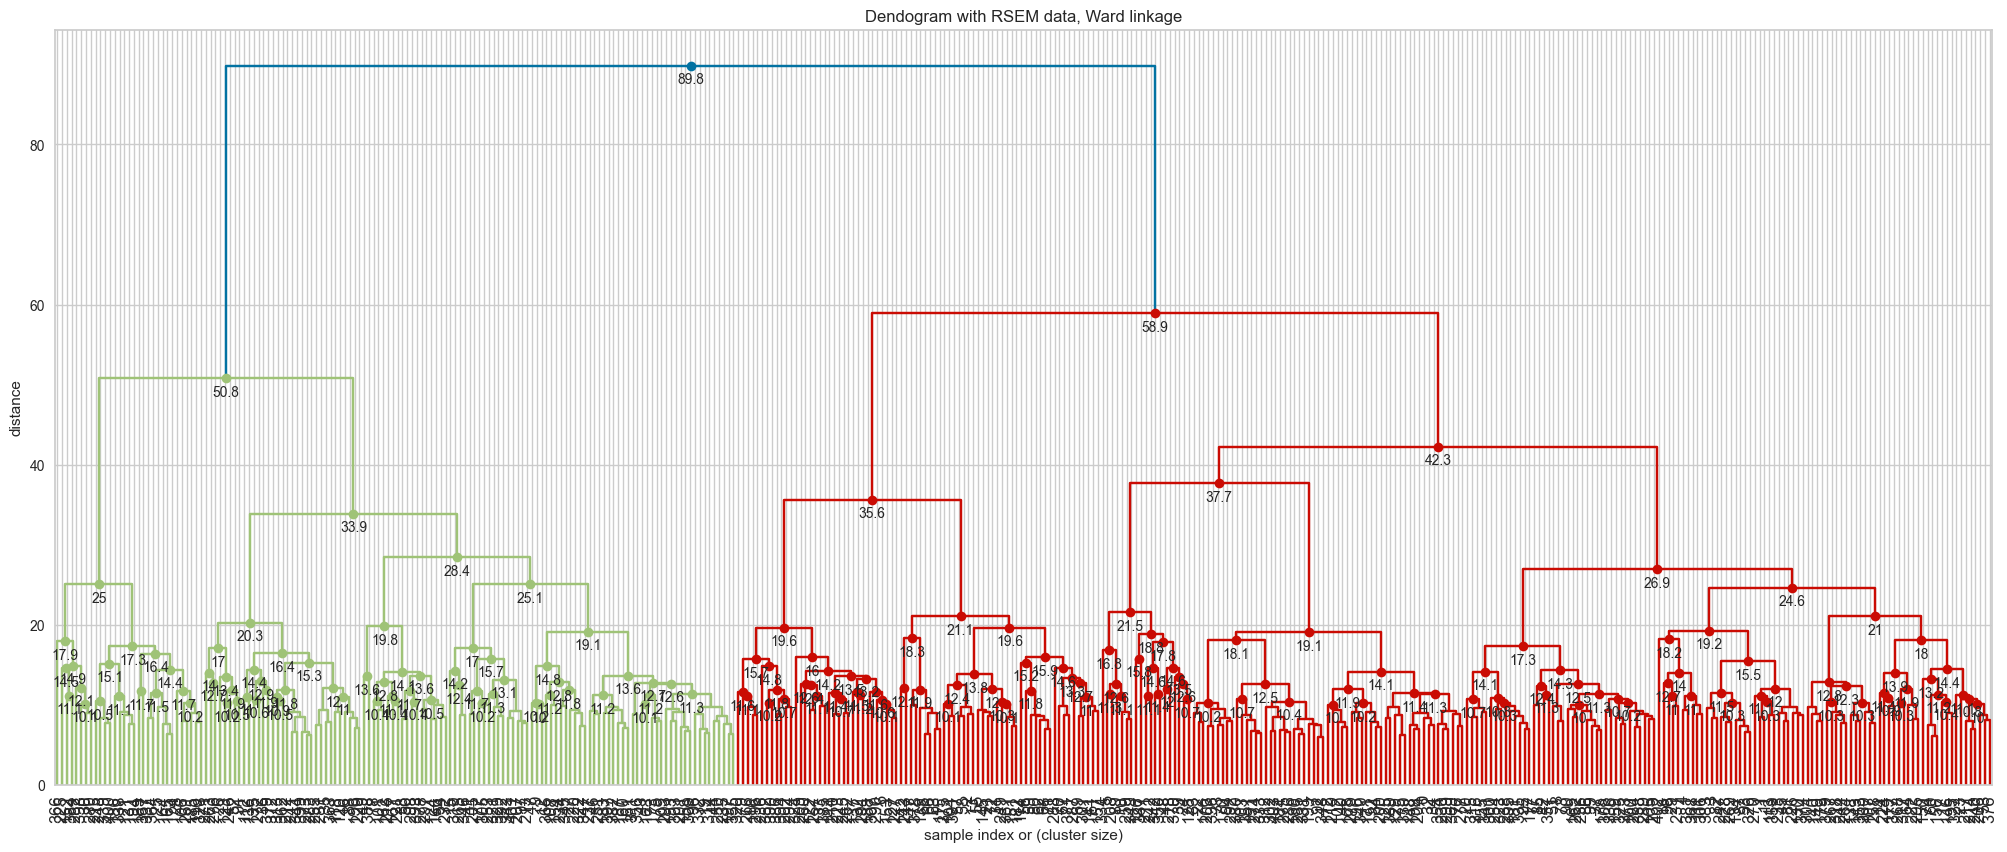
\includegraphics[width=1.0\textwidth,height=1.0\textheight,keepaspectratio]{Images/Clustering/dendogram.png}
      \caption{Dendogram specific to hierarchical clustering and it can be seen how the algorithm starts classifying each datapoint in its own cluster followed by a merge in higher up clusters. For this we have used the TCGA dataset for bladder cancer, using hierarchical clsutering with Ward linkage.}
      \label{fig:dendogram}
  \end{figure}
  \FloatBarrier




\end{appendices}